%! TEX root = ../main.tex
% ==============================================================
% IMMUTABLE — generated automatically, do not edit this block
%
% — Provenance ───────────────────────────────────────────────────
%   script            : analysis_scratch/damping_freq_overmooring.py
%   computed_in       : filters.py::damping_all_amplitude_grouper(collapse_panels=True) → plotter.py::_make_damping_freq_fig
%   plot_type         : damping_freq
%   data_class        : META
%   generated_at      : 2026-05-11T11:14:24
%   findings_doc      : 
%
% — Thesis context ──────────────────────────────────────────────
%   chapter           : 05
%   caption_label     : fig:ch05_damping_freq_overmooring
%   caption_short     : Transmisjon mot k, over-forankring. Tre figurer
%
% — Filters ────────────────────────────────────────────────────
%   panel             : all
%   wind              : allwind
%   amplitude [V]     : 0.1, 0.2, 0.3
%   frequency [Hz]    : 1.3, 1.6
%   probes            : 
%   run_category      : 
%   quality_flag      : 
%   mooring           : 
%
% — Data provenance ────────────────────────────────────────────
%   n_runs            : 24
%   in_probes_used    : 9373/170+9373/340, 9373/250
%   out_probes_used   : 12400/170+12400/340, 12400/250
%   probe_configs     : march2026_better_rearranging, nov_normalt_oppsett
%   non_final_config_n: 12
%   datasets        :
%     PROCESSED-20251112-tett6roof
%     PROCESSED-20251113-tett6roof
%     PROCESSED-20251113-tett6roof-loosepaneltaped
%     PROCESSED-20251113-tett6roof-probeadjusted
%     PROCESSED-20260307-ProbPos4_31_FPV_2-tett6roof
%     PROCESSED-20260312-ProbPos4_31_FPV_2-tett6roof
%     PROCESSED-20260313-ProbePos4_31_FPV_2-tett6roof
%     PROCESSED-20260314-ProbePos4_31_FPV_2-tett6roof
%     PROCESSED-20260316-ProbePos4_31_FPV_2-tett6roof
%     PROCESSED-20260316-ProbePos4_31_FPV_2-tett6roof-under9Mooring
%   run_paths       :
%     (omitted — aggregate over > threshold runs, see datasets)
%
% — Method / numerical parameters ─────────────────────────────
%   grouper           : damping_all_amplitude_grouper
%   collapse_panels   : True
%   fft_window_hz     : 0.1
%   extra_params      : window=0.1 Hz, amp_column='OUT/IN (FFT)' (paddle freq only); Mooring=above_50; PanelCondition in {full, reverse} pooled
%
% — Summary stats cited in caption ────────────────────────────
%   stat:median_fullwind_OUTIN : 0.6315
%   stat:median_nowind_OUTIN : 0.574
%   stat:n_panels     : 1
%   stat:n_amplitudes : 3
%   stat:n_total_points : 24
%   stat:n_runs_total : 79
%   stat:points_with_n1 : 4
%   stat:mooring      : above_50
%   stat:panel_pooling : full+reverse pooled (collapse_panels=True; justification: tab:app_panel_pooling)
%   stat:n_per_point_A1 : full-1.30Hz:n=6; full-1.40Hz:n=2; full-1.50Hz:n=1; full-1.60Hz:n=1; no-1.30Hz:n=16; no-1.40Hz:n=2; no-1.50Hz:n=3; no-1.60Hz:n=2
%   stat:n_per_point_A2 : full-1.30Hz:n=4; full-1.40Hz:n=2; full-1.50Hz:n=2; full-1.60Hz:n=2; no-1.30Hz:n=7; no-1.40Hz:n=2; no-1.50Hz:n=2; no-1.60Hz:n=3
%   stat:n_per_point_A3 : full-1.30Hz:n=5; full-1.40Hz:n=2; full-1.50Hz:n=2; full-1.60Hz:n=2; no-1.30Hz:n=7; no-1.40Hz:n=1; no-1.50Hz:n=2; no-1.60Hz:n=1
%
% — Subfigures available ───────────────────────────────────────
%     FIGURES/ch05_damping_freq_overmooring_A1.pdf
%     FIGURES/ch05_damping_freq_overmooring_A2.pdf
%     FIGURES/ch05_damping_freq_overmooring_A3.pdf
% ── end immutable block ─────────────────────────────────────────
\begin{figure}[p]
  \centering
  \begin{subfigure}[b]{1.0\linewidth}
    \centering
    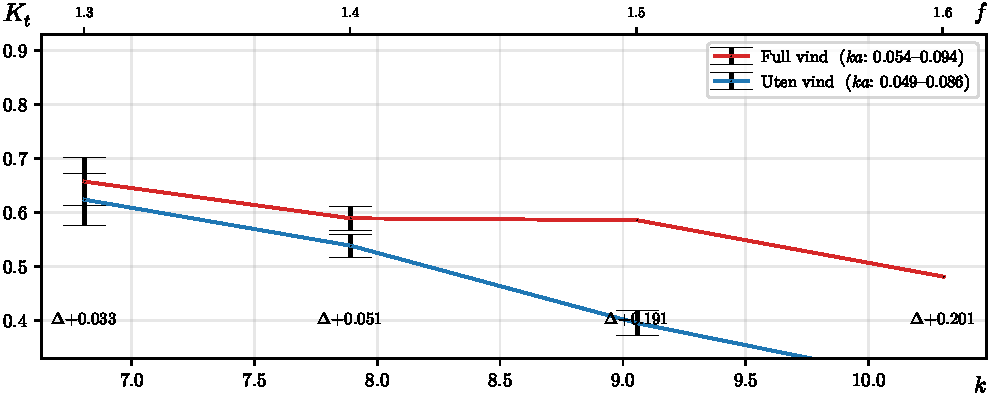
\includegraphics[width=\linewidth]{FIGURES/ch05_damping_freq_overmooring_A1.pdf}
    \caption{Over-forankring (above\_50, panel pooled), $A_1$}
    \label{fig:ch05_damping_freq_overmooring_A1}
  \end{subfigure}
  \\[1ex]
  \begin{subfigure}[b]{1.0\linewidth}
    \centering
    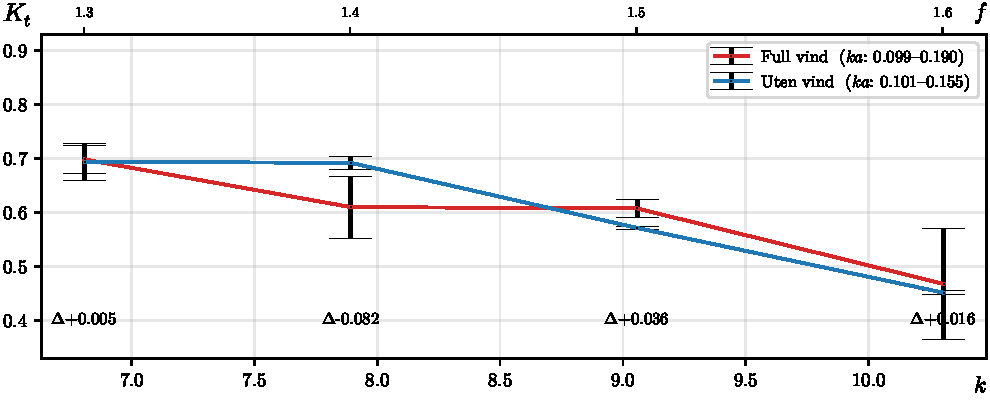
\includegraphics[width=\linewidth]{FIGURES/ch05_damping_freq_overmooring_A2.pdf}
    \caption{Over-forankring (above\_50, panel pooled), $A_2$}
    \label{fig:ch05_damping_freq_overmooring_A2}
  \end{subfigure}
  \\[1ex]
  \begin{subfigure}[b]{1.0\linewidth}
    \centering
    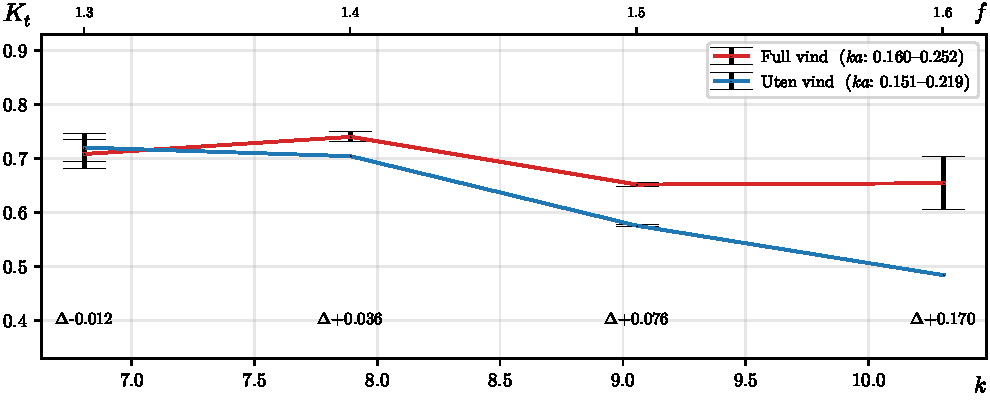
\includegraphics[width=\linewidth]{FIGURES/ch05_damping_freq_overmooring_A3.pdf}
    \caption{Over-forankring (above\_50, panel pooled), $A_3$}
    \label{fig:ch05_damping_freq_overmooring_A3}
  \end{subfigure}
% >>> CAPTION-SYNC START (do not edit this block; sync_captions.py overwrites)
  \caption[Transmisjon mot k, over-forankring. Tre figurer]{
    Transmisjonskoeffisient mot frekvens, over-forankring (above\_50). Helpanel og reverspanel slått sammen (begrunnelse: tab:app_panel_pooling). Usikkerhetsstolper viser standardavvik.
  }
% <<< CAPTION-SYNC END
  \label{fig:ch05_damping_freq_overmooring}
\end{figure}
